\documentclass[12pt]{amsart}
% ------------------------------------------------------------------------------
% Packages
% ------------------------------------------------------------------------------
\usepackage[utf8]{inputenc} % input encoding
\usepackage{framed} % for \framebox
\usepackage[english]{babel} % language support 
\usepackage[colorlinks=true, linkcolor=blue, urlcolor=blue, citecolor=blue, anchorcolor=blue]{hyperref} % hyperref package
\usepackage{amsthm, amsmath, amsfonts, mathtools, amssymb, bm} % Math packages
\usepackage{xcolor} % Color package
\usepackage[shortlabels]{enumitem} % Enumeration package
\usepackage{booktabs}
\usepackage{float}
\usepackage{cancel}

% ------------------------------------------------------------------------------
% Document Style
% ------------------------------------------------------------------------------

% Header ----------------------------------------------------------------------
\addtolength{\hoffset}{-2.25cm}
\addtolength{\textwidth}{4.5cm}
\addtolength{\voffset}{-2.5cm}
\addtolength{\textheight}{5cm}
\setlength{\parskip}{0pt}
\setlength{\parindent}{15pt}

\pagestyle{myheadings}

\setlength{\parindent}{0in}

\pagestyle{empty}
\makeatletter
\def\fps@figure{H}
\def\fps@table{H}
% ------------------------------------------------------------------------------

% ------------------------------------------------------------------------------
% New commands
% ------------------------------------------------------------------------------
\newcommand{\qiq}{\qquad \implies \qquad}
\newcommand{\qiffq}{\qquad \iff \qquad}
\newcommand{\qaq}{\qquad \textbf{and} \qquad}
\newcommand{\qoq}{\qquad \textbf{or} \qquad}

% ------------------------------------------------------------------------------
% New environments
% ------------------------------------------------------------------------------
\newtheorem*{theorem}{\color{red!60!black}Theorem}
\newtheorem{corollary}{\color{blue}Corollary}
\counterwithin*{corollary}{subsection}
\newtheorem{lemma}{\color{blue}Lemma}
\counterwithin*{lemma}{subsection}
\newtheorem{proposition}{\color{blue}Proposition}
\counterwithin*{proposition}{subsection} 
\theoremstyle{definition}
\newtheorem*{definition}{\color{green!60!black}Definition}
\newtheorem{example}{\color{orange!80!black}Example}
\newtheorem*{Obs}{\color{purple!80!white}Observation}
\newtheorem*{As}{\color{red!80!white}Assumptions}
\newtheorem*{answer}{\color{red!60!white}Answer}
\newtheorem*{Cor}{\color{blue!60!white}Corollary}
\newtheorem{exercise}{\color{blue!60!white}Exercise}
\newtheorem{subexercise}{ \color{blue!40!white}  }[exercise]

\begin{document}

\thispagestyle{empty}


{\scshape FIN-971} \hfill {\scshape \Large Problem Set \#1} \hfill {\scshape Fall 2021}\\
{\scshape Author(s): \hfill Mitchell Valdes-Bobes\\
{\scshape Date: \hfill \texttt{11/10/21}
\medskip

\hrule

\bigskip

\bigskip

\date{\today}

\begin{exercise}
  Following tables and figures are the result of computations using the code included in \href{https://github.com/mitchv34/FIN-971/blob/main/PS1/src/source.jl}{this repository}.


\section{Data}
\begin{center}
  \begin{tabular}{rr|ccccc}
\toprule
                                            &               & Obs & Mean     & Std. Dev. & Min      & Max       \\ \hline
      \multirow{4}{*}{EMS Technologies Inc} &         ppegt &  28 &   65.587 &    35.843 &    5.021 &   119.547 \\
                                            &     inv\_rate &  28 &    0.183 &     0.165 &    0.067 &     0.760 \\
                                            &    cash\_flow &  28 &    0.122 &     0.053 &    0.060 &     0.226 \\
                                            & tobin\_q\_lag &  28 &    0.885 &     1.569 &   -0.530 &     5.004 \\ \hline
      \multirow{4}{*}{Atwood Oceanics Inc.} &         ppegt &  28 &  351.544 &   256.491 &  126.435 &  1131.700 \\
                                            &     inv\_rate &  28 &    0.118 &     0.112 &    0.002 &     0.409 \\
                                            &    cash\_flow &  28 &    0.143 &     0.103 &   -0.029 &     0.350 \\
                                            & tobin\_q\_lag &  28 &    0.297 &     0.731 &   -0.423 &     2.382 \\ \hline
\multirow{4}{*}{Raytheon Technologies Corp} &         ppegt &  28 & 9498.077 &  3078.630 & 4092.137 & 15106.000 \\
                                            &     inv\_rate &  28 &    0.101 &     0.034 &    0.049 &     0.162 \\
                                            &    cash\_flow &  28 &    0.098 &     0.028 &   -0.016 &     0.126 \\
                                            & tobin\_q\_lag &  28 &    0.092 &     0.975 &   -0.999 &     2.007 \\
\bottomrule
\end{tabular}
\end{center}

\section{Plots}

\begin{figure}[h!]
  
  \centering
  
  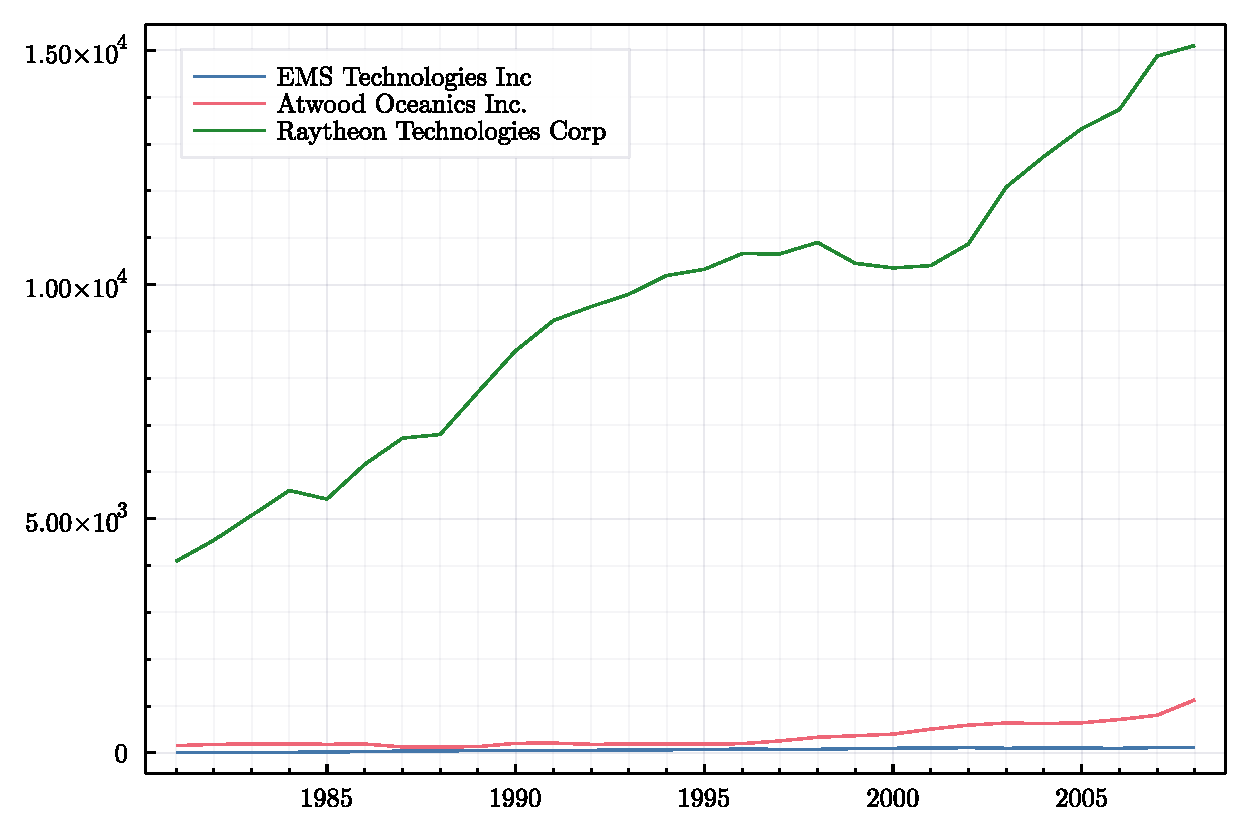
\includegraphics[scale=0.7]{figures/fig_1.pdf}

\end{figure}
\newpage
\begin{figure}[h!]\caption{EMS Technologies Inc.}
  
  \centering
  
  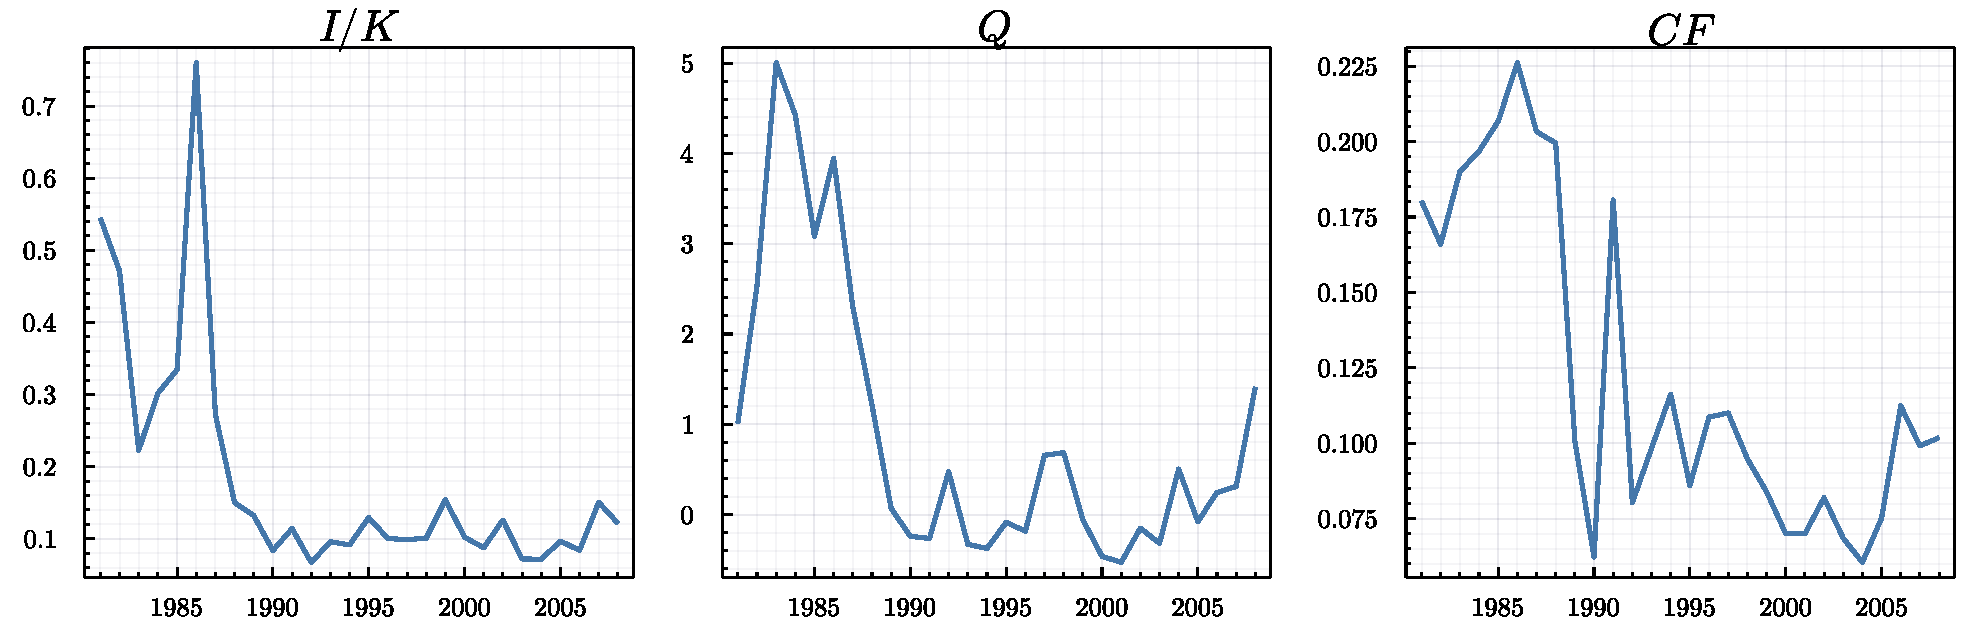
\includegraphics[scale=0.5]{figures/fig_2_EMS Technologies Inc.pdf}

\end{figure}


\begin{figure}[h!]\caption{Atwood Oceanics Inc.}
  
  \centering
  
  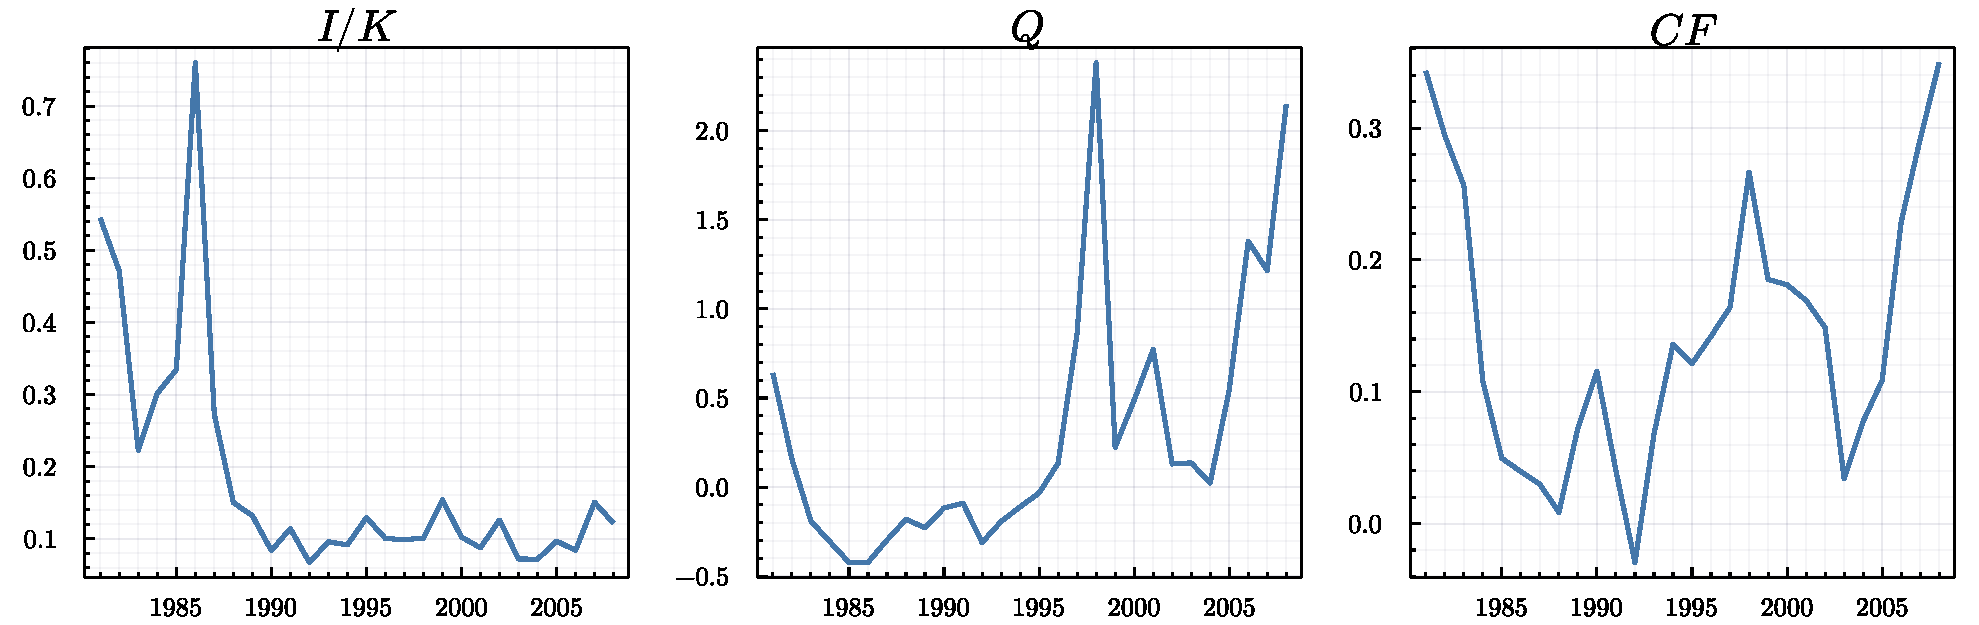
\includegraphics[scale=0.5]{figures/fig_2_Atwood Oceanics Inc..pdf}

\end{figure}

\begin{figure}[h!]\caption{Raytheon Technologies Corp.}
  
  \centering
  
  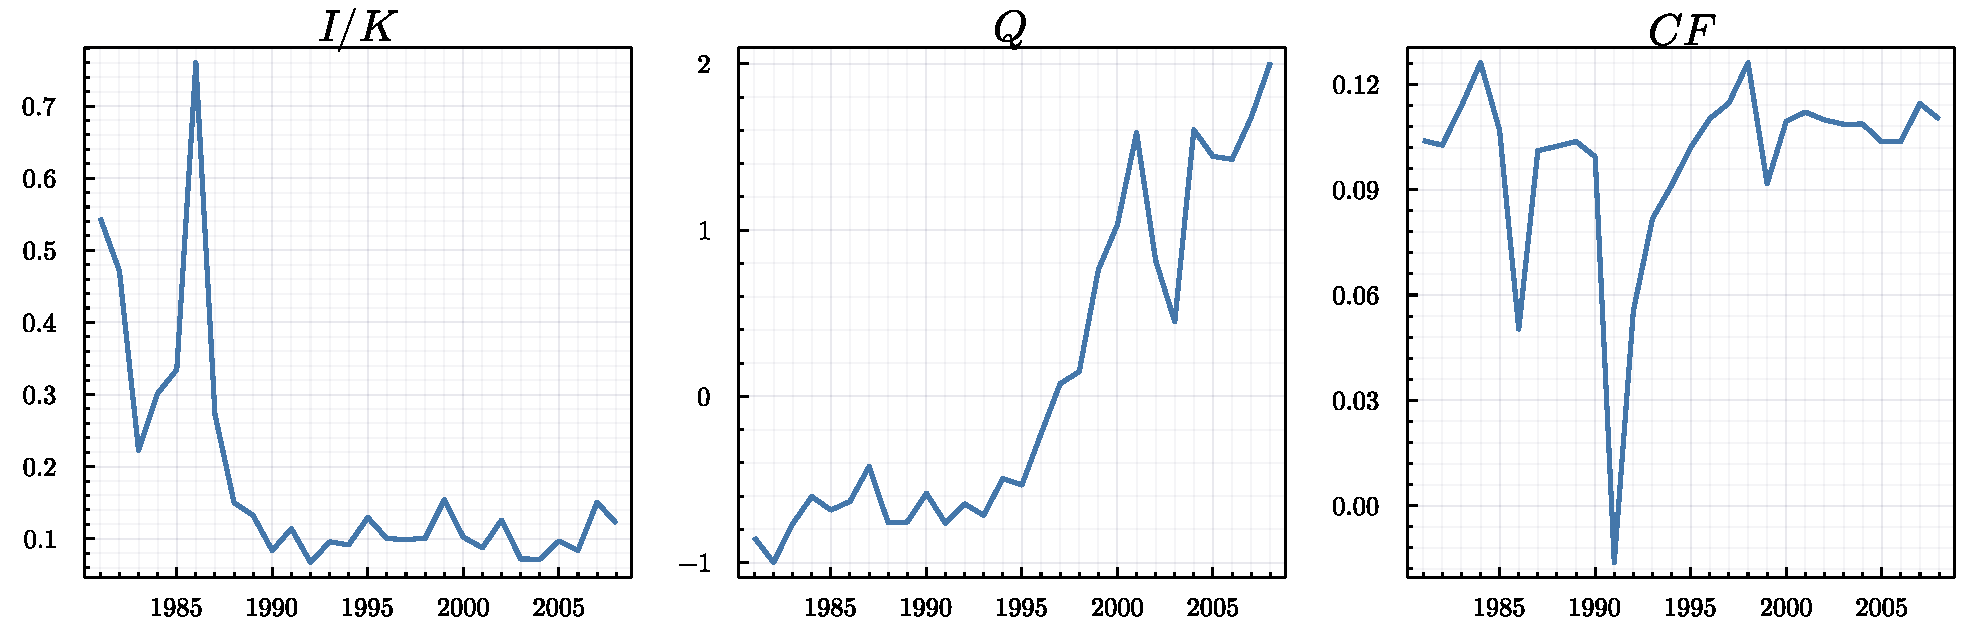
\includegraphics[scale=0.5]{figures/fig_2_Raytheon Technologies Corp.pdf}

\end{figure}

\newpage
\section{Regressions}
\subsection{$\beta_2 = 0$}
\begin{center}
  \begin{tabular}{r|ccc}
\toprule
              & EMS Technologies Inc & Atwood Oceanics Inc. & Raytheon Technologies Corp \\ \hline
  (Intercept) &             0.122*** &             0.083*** &                   0.103*** \\
              &              (0.027) &              (0.015) &                    (0.005) \\
tobin\_q\_lag &             0.070*** &             0.118*** &                  -0.024*** \\
              &              (0.015) &              (0.019) &                    (0.005) \\ \hline
            N &                   28 &                   28 &                         28 \\
        $R^2$ &                0.442 &                0.596 &                      0.457 \\
\bottomrule
\end{tabular}
\end{center}
\subsection{$\beta_2 \neq 0$}
\begin{center}
\begin{tabular}{r|ccc}
\toprule
              & EMS Technologies Inc & Atwood Oceanics Inc. & Raytheon Technologies Corp \\ \hline
  (Intercept) &               -0.041 &               0.048* &                   0.101*** \\
              &              (0.070) &              (0.025) &                    (0.019) \\
tobin\_q\_lag &                0.026 &             0.087*** &                  -0.024*** \\
              &              (0.022) &              (0.026) &                    (0.005) \\
   cash\_flow &              1.639** &                0.311 &                      0.026 \\
              &              (0.660) &              (0.185) &                    (0.192) \\ \hline
            N &                   28 &                   28 &                         28 \\
        $R^2$ &                0.552 &                0.637 &                      0.457 \\
\bottomrule
\end{tabular}
\end{center}

\end{exercise}



\end{document}